\documentclass[letterpaper]{article}

\usepackage{aaai}
\usepackage{times}
\usepackage{helvet}
\usepackage{courier}
\usepackage{graphicx}
\usepackage{stfloats}
\usepackage{color}

% \usepackage{float}
% \floatstyle{boxed} 
% \restylefloat{figure}

\usepackage[noend,linesnumbered,algoruled]{algorithm2e}
% %%%%%%%%%%%%%%%%%%%%%%%%%%%%%%%%%%%%%%%%%%%%%%%%%%%%%%
% PDFMARK for TeX and GhostScript
% Uncomment and complete the following for metadata if
% your paper is typeset using TeX and GhostScript (e.g
% if you use .ps or .eps files in your paper):
% \special{! /pdfmark where
% {pop} {userdict /pdfmark /cleartomark load put} ifelse
% [ /Author (John Doe, Jane Doe)
% /Title (Paper Title)
% /Keywords (AAAI, artificial intelligence)
% /DOCINFO pdfmark}
% %%%%%%%%%%%%%%%%%%%%%%%%%%%%%%%%%%%%%%%%%%%%%%%%%%%%%%
% PDFINFO for PDFTeX
% Uncomment and complete the following for metadata if
% your paper is typeset using PDFTeX
% \pdfinfo{
% /Title (Input Your Title Here)
% /Subject (Input The Proceedings Title Here)
% /Author (First Name, Last Name;
% First Name, Last Name;
% First Name, Last Name;)
% }
% %%%%%%%%%%%%%%%%%%%%%%%%%%%%%%%%%%%%%%%%%%%%%%%%%%%%%%
% Uncomment only if you need to use section numbers
% and change the 0 to a 1 or 2
% \setcounter{secnumdepth}{0}
% %%%%%%%%%%%%%%%%%%%%%%%%%%%%%%%%%%%%%%%%%%%%%%%%%%%%%%


\newcommand{\from}[2]{\textcolor{red}{\noindent\textbf{//}\textbf{Note
      from #1:}\textsc{ #2}\textbf{//}}}
      
      \newcommand{\fw}[1]{\texttt{#1}}




\begin{document}

\title{Towards a Cognitive System That Can Recognize Spatial Regions Based on Context}
% \title{Representing and Reasoning About Spatial Regions Defined by Context}
% \title{Context-Dependent Spatial Regions}

\author{}


\maketitle
\begin{abstract}
In order to collaborate with people in the real world, cognitive systems must be able to represent and reason about spatial regions in human environments. Consider the command \emph{``go to the front of the classroom''}. The spatial region mentioned (the front of the classroom) is not perceivable using geometry alone. Instead it is defined by its functional use, implied by nearby objects and their configuration. In this paper, we define such areas as \textit{context-dependent spatial regions} and propose a method for a cognitive system to learn them incrementally by combining qualitative spatial representations, semantic labels, and analogy. Using data from a mobile robot, we generate a relational representation of semantically labeled objects and their configuration. Next, we show how the boundary of a context-dependent spatial region can be defined using \textit{anchor points}. We then demonstrate how an existing computational model of analogy can be used to transfer this region to a new situation. To evaluate this process we compare transferred regions to annotations made on maps of real rooms by human volunteers.
\end{abstract}

 \section{Introduction}

Consider a janitorial robot cleaning a classroom. While performing this task, it encounters a teacher working with a student. The teacher tells the robot to ``start at the front of the classroom'', expecting it to go to the front of the classroom and begin cleaning that area. This response requires that the robot is able to \emph{determine the spatial region in the environment that satisfies this concept}.

The ability to understand and reason about \textit{spatial regions} is essential for cognitive systems performing tasks for humans in everyday environments. Some regions, such as whole rooms and corridors, are defined by clearly perceivable boundaries (e.g. walls and doors). However, many regions to which humans routinely refer are not so easily defined. Consider, for example, the aforementioned region \textit{the front of the classroom}. This region is not easily perceivable using just the geometry of the environment. Instead, it is defined by the objects present in the room (chairs, a desk, a chalkboard), their role in this context (seats for students to watch a teacher who writes on the chalkboard) and their configuration in space (the seats point toward the chalkboard). In this paper, we will refer to such regions as \textit{context-dependent spatial regions} (CDSRs). 

% nah: These are the main claims from the ACS paper, but they can be reduced/dropped for aaai

Representing and reasoning about context-dependent spatial regions is beyond the capabilities of current cognitive systems, yet it is an important ability for three reasons:

\begin{itemize}

\item{If cognitive systems are to collaborate with humans in everyday environments, then they must be able to represent and reason about the spatial regions humans refer to. Many regions are best defined in a context-dependent manner, for example, a kitchen in a studio apartment, an aisle in a church or store, behind enemy lines in a military engagement, etc.}


\item{Cognitive systems must integrate different types of information, including geometric, semantic, and functional knowledge. The identification of context-dependent spatial regions provides a suitable task for studying this integration. 
% Only through such integration could a system determine, for example, whether a banquet hall has a dancefloor depending on the arrangement of the room.
}

\item{Cognitive systems must adapt their knowledge and experience to new situations. While humans do not demonstrate mastery after seeing a single example of a new concept, they are able to begin using it immediately, whilst incrementally refining it over time (cf. one-shot learning~\cite{Fei-Fei/etal:2006}). This has important implications with respect to the amount of knowledge engineering and training time required to create a cognitive system. For example, having trained a mobile robot to understand the front of one classroom, it is desirable for it to be able to identify the front of other classrooms and similar areas (e.g. theaters) without additional tutoring.}
\end{itemize}

% nah: removed large motivating picture, hoping we can make do with just our result pictures, or replace it with images used for ground truth

This paper presents a novel integration of technologies which allows an artificial cognitive system (specifically a mobile robot) to represent and reason about CDSRs. Our approach is founded on two assumptions. The first assumption is that CDSRs can be defined using qualitative spatial representations (QSRs) extracted from the sensor data of the system~\cite{Cohn:2001}. The second assumption is that semantically similar areas (e.g. two different classrooms) will feature similar CDSRs, and that these similarities can be recognised through analogy. The rest of the paper is structured following these assumptions. Section~\ref{sec:qsr-gen} describes how we generate QSRs from sensor data taken from an existing, state-of-the-art, cognitive system and use these to define CDSRs. Section~\ref{sec:analogy} then describes how use the structure-mapping model of analogy \cite{Gentner1983a} to transfer a CDSR from a labelled example to a new situation. Section~\ref{sec:example} presents a worked example of the entire process, and Section~\ref{sec:evaluation} evaluates our system in comparison to data from human subjects performing the same task.


\section{From Sensors to Qualitative Representations}\label{sec:qsr-gen}

% Our approach to representing and reasoning about context-dependent spatial regions requires the existence of qualitative spatial representations~\cite{Cohn:2001} describing the relationships between the entities a cognitive system perceives (including objects, groups, and regions). By adding semantic labels, or types, to each entity, we are able to reason about the geometric \emph{and} conceptual characteristics of the system's environment. The following sections describe how we generate appropriate qualitative spatial representations using the spatial model of an existing, state-of-the-art, cognitive system.

The context which defines a CDSR is a combination of the functional and geometric properties of a room, i.e. what can be done there and where. In this work we implicitly represent context using the types of objects present in a room and their location, both relative to each other and relative to the room itself. The following sections describe how we construct these ingredients of context from the starting point of a robot that can sense its environment. 

\subsection{The Dora System}

We base our work on Dora, a mobile cognitive robot with a pre-existing multi-layered spatial model~\cite{Hawes/etal:2011}. In this paper, we draw on the metric map from this model. For more information on Dora's other competences, see recent papers, e.g.~\cite{Hawes/etal:2011,Hanheide/etal:2011}.

Dora's metric map is a collection of lines in a 2D global coordinate frame. These lines are generated by a process which uses input from the robot's odometry and laser scanner to perform simultaneous localization and mapping (SLAM). Lines in this SLAM map represent features extracted from laser scans wherever a straight line is present for long enough to be considered permanent. In practice, lines are generated at the positions of walls and any other objects that are flat at the height of the laser (e.g. bins, closed doors etc.). The robot's location in the metric layer is represented as a 2D position plus an orientation. 

Dora is capable of using vision to recognize pre-trained 3D object models. Recognition can either be triggered through autonomous visual search or at a user's command. When an object is detected it is represented in the metric map 
by placing a copy of the model at the detected pose. The recognizer associates each object with a type label that was provided during a training phase.  

To enable us to generate a range of different evaluation situations in a reasonable length of time, we have generated data from Dora in both real rooms and in simulation. Simulation is performed using the Player/Stage hardware abstraction layer~\cite{GerkeyVaughanHoward03} allowing us to run the system \emph{mostly unchanged} in a pre-defined environment. Also, to enable us to detect a wider range of objects than is usually possible (from armchairs to whiteboards), we used a simulated object recogniser in all runs. The recogniser was configured with types and positions of objects in the environment and was guaranteed to detected them when the robot was orientated towards them. This eliminated any errors from the recognition process, but was still influenced by errors in robot localisation. 

\subsection{Qualitative Spatial Representation Extraction}

JK working on this!

%Given data from Dora's spatial model, we compute the following qualitative spatial representations. First, we extract the object and room entities from the sensor data. Next, we determine the qualitative spatial relationships between these entities. For the room, we compute its region as a convex hull around the set of points. For the objects, we consider only their centroids. For each pair of adjacent objects, we compute topological and positional relationships. Adjacency is determined by creating a voronoi diagram as is standard geometric reasoning \cite{Forbus/etal2003}. For the topological relationships, we use the region connection calculus, RCC8, \cite{Cohn:2001}. For positional relations, we use two predicates \fw{leftOf} and \fw{below}. An entity is \fw{leftOf} another if the x coordinate of its centroid is less than that of the other entity's. An entity is \fw{below} another if the y coordinate of its centroid is less than that of the other entity's. Objects whose x or y coordinates are within a threshold of one another will not be related by \fw{leftOf} or \fw{below} positional relations.

%%\from{Nick}{I have changed the below paragraph to match the actual numbers and images. I've marked what I changed}
%%Desk 1 and Desk 2 are not labeled in the Figure.

%Consider the situation in Figure~\ref{fig:dora-spatial} where the robot is facing two desks in a row\footnote{Please note that although the desks in front of the robot in Figure~\ref{fig:dora-spatial} appear distributed left to right from the robot's current position, they are actually distributed bottom to top, according to our definitions, in the global coordinate frame.}. Because we represent the desks as distinct points, \fw{(rcc8-DC Desk1 Desk2)} states that they are disjoint. To account for their relative positions, neither \fw{(leftOf Desk1 Desk2)} nor \fw{(leftOf Desk2 Desk1)} are true because the x coordinate of \fw{Desk1} is within a threshold of the x coordinate of \fw{Desk2}. The statement \fw{(below Desk1 Desk2)} is true because \fw{Desk1} has a lower y coordinate. Each desk is also related to the room by the non-tangential proper part relation, \fw{rcc8-NTPP}. These qualitative spatial relationships provide the structure necessary for analogical processing.


\subsection{Representing Context-Dependent Spatial Regions}

We use \textit{anchor points}~\cite{Klenk/etal2005} to define the boundaries of CDSRs. Anchor points are symbolic descriptions which link a conceptual entity (i.e. something that can be reasoned about but not directly perceived, such as a CDSR) to a particular point on a perceived entity. The perceived entities we use are the objects recognised by Dora, and the room itself. The room representation is created by putting a convex hull around the lines in Dora's SLAM map. Anchor points are created from perceived entities using unary functions, e.g. \fw{(CentroidFn Desk1)} represents the centroid of the geometric extent of \fw{Desk1}, and are linked to a particular CDSR using a \fw{regionBoundary} relation. After we have defined the boundary of the region, we assign it a semantic label using the \fw{regionType} relation. Therefore, each CDSR has one type and a variable number of boundary points.


\from{Nick}{TODO: Need to update example, including new fns, when we have updated pictures in.}

\begin{figure}[h]
	{\fontsize{8}{8} %%Because aaai.sty overrides usual font size commands
  
\fw{(regionType CDSR1 FrontRegion)\\
(regionBoundary CDSR1 (LeftmostTopFn Room1))\\
(regionBoundary CDSR1 (LeftmostBottomFn Room1))\\
(regionBoundary CDSR1 Desk1)\\
(regionBoundary CDSR1 Desk2)\\
(regionBoundary CDSR1 Desk3)\\
(regionBoundary CDSR1 Desk4)\\
(regionBoundary CDSR1 Whiteboard0)\\
}}
  \caption{Representing the front of the classroom context-dependent region \fw{CDSR1}}
  \label{fig:cdsr-reps}
\end{figure}

Figure \ref{fig:cdsr-reps} contains the symbolic description for the front of classroom \fw{Room1} which is pictured in the top of Figure~\ref{fig:rooms}. The anchor points (connected in orange in Figure~\ref{fig:rooms}) define the region. \fw{(LeftmostBottomFn Room1)} and \fw{(LeftmostTopFn Room1)} are the points with the lowest x coordinate out of the set of points defined as the top and bottom of \fw{Room1} respectively. The sets of points representing the top and bottom of the classroom are found by selecting the points defining the area within a threshold of the area's maximum or minimum y coordinate. The other corners of the context-dependent spatial region are defined by the four desks and the whiteboard. Because perceived objects (e.g. the desks) are defined as single points, they can serve as anchor points directly. The semantic label \fw{FrontRegion} ties the geometric extent of the boundary points to a conceptual region. This definition for the front of the classroom is specific to \fw{Room1} and its entities. It is clearly context-dependent because its extent is dependent on the arrangement of the anchor points used to define its boundary. If the desks were in a different position then the region would cover a different extent (e.g. if they were closer to the whiteboard then the region would be smaller). 



\section{Analogical Transfer of Spatial Regions}\label{sec:analogy}

% \from{Nick}{This section feels a bit long. Can we cut it down at all? Perhaps the second half of the second paragraph if we don't use the constraints explicitly}
% done

We assume that a cognitive system will have a way of initially acquiring examples of CDSRs, e.g., by being taught through dialogue, sketching, or hand-coding. To avoid burdening potential tutors with the task of teaching the system every CDSR individually, it is desirable for a cognitive system to be able to automatically recognize similar regions after initial training. For example, after a janitorial robot has been taught where the front of one classroom is, it should be able to identify the fronts of other classrooms in the building. We have chosen \emph{analogy} as the approach our system will use to solve this problem, as analogy has been previously used to successfully combine semantic as well as geometric information in spatial reasoning tasks~\cite{Lockwood/etal2008}.


Analogy is an essential cognitive process. In humans, analogical processing has been observed in language comprehension, problem-solving, and generalization \cite{Gentner2003}. The structure-mapping theory of analogy and similarity postulates this process as an alignment between two structured representations, a \textit{base} and a \textit{target} \cite{Gentner1983a}. 
% This alignment process is governed by three constraints: \textit{identicality}, \textit{parallel connectivity}, and \textit{one-to-one mapping}. The identicality constraint provides a strong preference for only allowing identical predicates to match. Parallel connectivity states that if two predicates are matched then their arguments must also match. The one-to-one mapping constraint requires that each element in the base corresponds to at most one element in the target and vice versa. To select between competing mappings, the \textit{systematicity} principle prefers mappings that are highly interconnected and contain deep chains of higher order relations over mappings with an equal number of relations which are independent from each other.
We use the Structure-Mapping Engine (SME) \cite{Falkenhainer1989a} to perform analogical matching in our system. Given base and target representations as input, SME produces one or more mappings. Each mapping is represented by a set of \textit{correspondences} between entities and expressions in the base and target structures.  Mappings also include \textit{candidate inferences} which are conjectures about the target using expressions from the base which, while unmapped in their entirety, have subcomponents that participate in the mapping's correspondences. SME operates in polynomial time, using a greedy algorithm \cite{Forbus/etal1994}.

\begin{figure}[h]
  \includegraphics[width=\columnwidth]{analogy2.png}
  \caption{Analogical mapping between four base expressions and two target expressions. Ovals and squares represent relations and entities respectively. Purple dashed bi-directional arrows are the correspondences between the base and target, and the green dashed arrow, oval, and square represent a candidate inference projected into the target.}
  \label{fig:analogy}
\end{figure}

\from{Nick}{TODO: Update Figure \ref{fig:analogy} with correct representation for current version.}

Figure \ref{fig:analogy} illustrates a sample mapping between four base expressions and two target ones. Each oval represents a binary predicate, and its two entity arguments are represented by squares. SME generates a mapping between the base expressions \fw{(rcc8-DC Desk1 Desk2)} and \fw{(below Desk1 Desk2)}, and the  target expressions \fw{(rcc8-DC Desk20 Desk22)} and \fw{(below Desk20 Desk22)}. This is done in the following manner. First, the predicates of these expressions are placed in correspondence by the identicality constraint. Next, parallel connectivity aligns their arguments, \fw{Desk1} with \fw{Desk20} and \fw{Desk2} with \fw{Desk22}. While there is another \fw{below} statement in the base about two desks, it cannot correspond to either of the target expressions in the same mapping due to the one-to-one constraint. In Figure \ref{fig:analogy}, these correspondences are highlighted by the purple hashed bi-directional arrows. Next, SME creates a candidate inference for the expression \fw{(regionBoundary CSDR1 Desk1)}, because \fw{Desk1} participates in the mapping. The candidate inference is stated as \fw{(regionBoundary (:skolem CSDR1) Desk20)}. \fw{:skolem} is used to denote entities that do not exist in the target description but are included in the candidate inferences. In this case, the candidate inference states that there is something like \fw{CSDR1} in the target, and its boundary includes \fw{Desk20}. Note that inference is selective, with no candidate inferences generated for the entirely unmapped \fw{below} expression. Next, we describe how we use the results of an analogy to infer a context-dependent spatial region in the target.
 
% It feels odd having this as a separate subsection
%\subsection{Initial Approach}\label{sec:approach}

In our system, the base and target representations consist of the entities Dora has perceived in two different rooms, plus the QSRs computed on top of these. The base also contains a labeled CDSR which we assume is sought in target. The result of result of running SME on these representations is a set of correspondences between the base and target, and a set of candidate inferences about the target. We use these to transfer the CDSR from base to target (i.e. recognizing the CDSR in the target) as follows. First, we identify the CDSR of the sought type in the base. This entity should not participate in the mapping, but should be included in \fw{:skolem} expressions in the candidate inferences. To transfer the CDSR to the target, we collect the candidate inferences that result from \fw{regionBoundary} statements mentioning the base CDSR. The second arguments of these candidate inferences are anchor points in the target environment. We use these to define the boundary of the CDSR in the target, linking them to a new CDSR entity using \fw{regionBoundary} statements. 

\section{Example System Run}\label{sec:example}


% all images in a single figure -- pretty ugly and a waste of space
% \begin{figure*}[t]
%   \includegraphics[width=\textwidth]{images/worked-example.png}
%   \caption{\textbf{TODO}}
%   \label{fig:rooms-and-pic}
% \end{figure*}


\begin{figure}
  \includegraphics[width=\columnwidth]{images/worked-example-rooms.png}
  \caption{Maps of 2 real classrooms generated by our system, plus an expert-annotated CDSR (orange, top image), subject-annotated CDSR (red, bottom image) and a CDSR transferred by analogy (green bottom image). The classroom used to generate the top classroom is pictured in Figure~\ref{fig:ug40}}
  \label{fig:rooms}
\end{figure}

\begin{figure}
  \includegraphics[width=\columnwidth]{images/ug40.png}
  \caption{One of the classrooms used in our evaluation. This image was presented to subjects who were  asked to annotate a copy of the image in the bottom half of Figure~\ref{fig:rooms}.}
  \label{fig:ug40}
\end{figure}



To elucidate the workings of our system, we now present an example of how it can transfer a CDSR describing the front of a known classroom (the base) to a new classroom (the target). 

We first create the base and target representations by running Dora in the two different classrooms. These are pictured in the top and bottom of Figure~\ref{fig:rooms} respectively. In each case, Dora is manually driven around the room to allow it to create a metric map. Once the map is created, Dora is then positioned such that the objects are observable and the visual recognition system is run. The map and object data that results from this is then passed on to the QSR generator. In the base case Dora perceives 2 desks, a whiteboard and the room area. To this we add the CDSR representing the front of the room. The case includes a total of \textbf{SOMENUMBER} expressions relating the \textbf{SOMENUMBER} entities. \textbf{SOMENUMBER} of these expressions are used to define the boundary of a CDSR representing the front of the room: the \textbf{SOMENUMBER} desks in the front row, the whiteboard, and the leftmost bottom and leftmost top of the room. The target case includes \textbf{SOMENUMBER}. The target case includes \textbf{SOMENUMBER} statements and \textbf{SOMENUMBER} entities.

SME generates an analogy between the base and target cases enabling the transfer of the symbolic description of the front of the room to the new situation. The resulting analogy includes \textbf{SOMENUMBER} correspondences between the entities and expressions in the base and target and \textbf{SOMENUMBER} candidate inferences.  All \textbf{SOMENUMBER} \fw{regionBoundary} statements in the base appear as candidate inferences. \textbf{SOMENUMBER} of the anchor points are exactly correct, the \textbf{\dots}. The other \textbf{SOMENUMBER} analogically transferred anchor points are to the \textbf{\dots}. The green region in the lower image of Figure \ref{fig:rooms} illustrates the CDSR created by the \textbf{SOMENUMBER} boundary points in the target environment. 


% coming soon


The implementation of the continual planning and switching parts is
based on MAPSIM \cite{brenner:nebel:jaamas09} and is able to use
several planners as the underlying planning system. We use a modified
version of Fast Downward \cite{fast-downward}, which we extended with
the support for actions with success probabilities. Finally, we use
\system{dlib-ml} \cite{king:2009} for successive estimation of the
underlying belief-state.

The baseline approach is using the same continual planning system as
the switching planner, but instead of creating an observation problem
for the decision theoretic planner it will just execute one sensing
action -- assuming that this action will confirm its assumption.

To test our approch we use a robot exploration domain similar to the
one used on a physical robotic system. It involves a robot exploring
an office or living environment and trying to return objects to their
owner.

\begin{figure}[h]
  \centering
  %\documentclass[letterpaper]{article}

% \begin{document}
% \pagestyle{empty}
  \tikzstyle{key} = [diamond, draw=black, inner sep=1pt]
  \tikzstyle{door} = [line width=4pt, draw=white]
  \tikzstyle{robot} = [circle, draw=black, fill=black!50, inner sep=2pt, minimum size=0.4cm]
  \tikzstyle{place} = [circle, draw=black, inner sep=2pt]
  \tikzstyle{roomlabel} = [inner sep=0.5pt]
  \begin{tikzpicture}

    \draw (0, 0) rectangle (4.3, 1.6);
    \draw (0, 1.6) rectangle (2.5, 3.0);
    \draw (2.5, 1.6) rectangle (4.3, 3.0);
    \draw[door] (1.3, 1.6) -- (1.9, 1.6);
    \draw[door] (2.9, 1.6) -- (3.5, 1.6);

    \node[place] (p1a) at (2.4, 0.8) {};
    \node[place] (p2a) at (1.6, 1.2) {}
      edge (p1a);
    \node[place] (p3a) at (3.2, 1.3) {}
      edge (p1a);
    \node[place] (p4a) at (3.8, 0.4) {}
      edge (p3a);
    \node[place] (p5a) at (2.7, 0.3) {}
      edge (p4a)
      edge (p1a);
    \node[place] (p6a) at (0.7, 0.5) {}
      edge (p1a)
      edge (p2a);


    \node[place] (p1b) at (1.6, 2.0) {}
      edge (p2a);
    \node[place] (p2b) at (1.8, 2.7) {}
      edge (p1b);
    \node[place] (p3b) at (0.3, 2.7) {}
      edge (p2b);
    \node[place] (p4b) at (0.3, 2.0) {}
      edge (p3b)
      edge (p1b);

    \node[place] (p1c) at (3.2, 2.0) {}
      edge (p3a);
    \node[place] (p2c) at (3.7, 2.7) {}
      edge (p1c);
    \node[place] (p3c) at (2.8, 2.6) {}
      edge (p2c)
      edge (p1c);
      

    \node[roomlabel, anchor=south west] (room0) at (0,0) {$\mathit{room}_A$};
    \node[roomlabel, anchor=south west] (room1) at (0,1.6) {$\mathit{room}_B$};
    \node[roomlabel, anchor=south east] (room2) at (4.3,1.6) {$\mathit{room}_C$};


    % \node[anchor=north west] (door1) at (0.25, 2) {$\mathit{door}_1$};
    % \node[anchor=north west] (door2) at (2.7, 2) {$\mathit{door}_2$};

    \node[robot] (robot) at (2.2, 1.0) {};


  \end{tikzpicture}
% \end{document}                  

%%% Local Variables: 
%%% mode: latex
%%% TeX-master: "../moritz_2011"
%%% End: 

  \caption{A exploration domain with three rooms and 13 places. The
    robot is in in the center of room A}
\label{fig:dora2}
\end{figure}
An instance of this domain is shown in figure \ref{fig:dora2}. The
basic building blocks of the domain consist of {\tt rooms}, {\tt
  places} and {\tt objects}. Places are grouped in rooms and objects
(as well as the robot) are always in a place. The robot can move
around the rooms via connections between places given by the {\tt
  connected} predicate. Each room has a (possibly unknown) {\em
  category/} (e.g. kitchen, office, living room) and depending on this
category, objects are placed inside the rooms.

The robot can find out if an object is at a certain place by executing
the {\tt look-for-object} action, which may result in a perception if
the object is in fact there (though some objects are harder to detect
than others -- so absence of a percept is no proof of the object's
absence). Additionally, if the robot is in the presence of a human, it
may simply ask what type of room they are currently in -- but
conducting a dialogue is a bit more costly than simply running the
vision algorithm (cost of 8 vs costs of 3).

We conducted experiments on scenarios of several sizes. The robot's
goal was to find one or more objects and report back their position to
a person. In order to determine the impact of sensor reliability on
both approaches, we also ran tests on identical problems but changed
the sensor model for the goal objects: the probability for percieving
the object if it was there went from 0.9 in the easiest case to 0.65
and 0.4 in the average and hard cases. In addition, we wanted to test
how our system performed on tasks requiring indirect sensing, so we
gave the planner goals to visit a certain type of room (e.g. kitchen
or office). We didn't place any humans in those scenarios, so the only
way of determining the room category was by looking for objects
typical for that room type. As this indirect reasoning is a tasks that
cannot be performed by the continual planner alone, we did not run the
baseline system on those problems.

As the initial state of the problems is stochastic, we ran 50
simulations for each configuration. The samples for the true initial
state were drawn from the same distribution that was used for
planning, so the planner's model matched its simulated world
exactly. Not all problems generated in this manner have a solution. We
did not reject these problems, as we believe that detecting the
non-existance of a solution is important in stochastic domains.


Fast Downward was run with the cyclic causal graph heuristic using A*
search or weighted A* with a weight of 5, depending on the difficulty
of the problem. We then performed multiple tests with different limits
for the belief space size of the decision theoretic subtask. Higher
limits should cause longer planning times but be beneficial to plan
quality as more contingencies can be taken in to account by the POMDP
planner.

Using a satisficing, optimistic serial planner and using continual
planning makes optimising for the expected reward difficult. The
continual planner will in general be overly optimistic regarding the
remaining costs to the goal while being overly pessimistic regarding
the probability of reaching it (as it only regards one trace). This
means that setting the reward function to non-extremal setting had
little effect on the resulting planner behaviour. For this reason, we
chose not to use the expected reward as a metric for our results, as
that information would have been of little value to the
reader. Instead we show the average costs of the plan and the success
rate (as a ratio between solved and solvable problems) separately.

\begin{figure}[h!]
  % \centering
  % 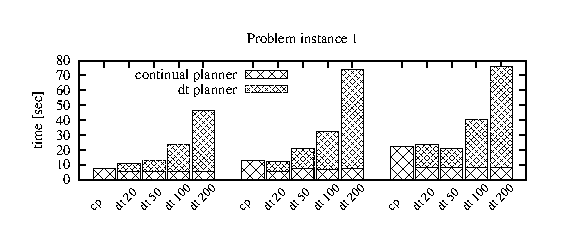
\includegraphics{dora1-time}\hfill
  % \vspace{2mm}
  \includegraphics{dora2-time}\hfill
  \vspace{2mm}
  \includegraphics{dora3-time}\hfill
  \vspace{2mm}
  \includegraphics{dora4-time}\hfill
  \vspace{2mm}
  \includegraphics{dora56-time}\hfill
  \vspace{2mm}
  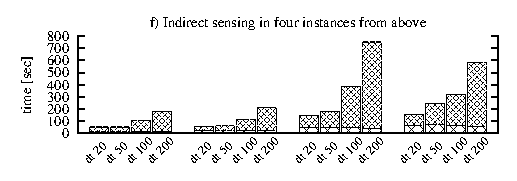
\includegraphics{dora-cat-time}\hfill
  \caption{Average runtime}
  \label{fig:results-time}
\end{figure}

\begin{figure}[h!]
  % \centering
  % \includegraphics{dora1-quality}\hfill
  % \vspace{2mm}
  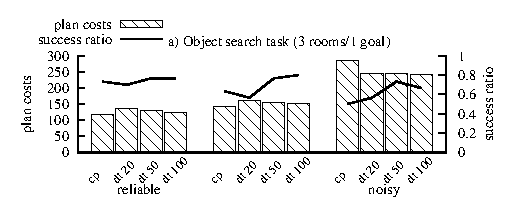
\includegraphics{dora2-quality}\hfill
  \vspace{2mm}
  \includegraphics{dora3-quality}\hfill
  \vspace{2mm}
  \includegraphics{dora4-quality}\hfill
  \vspace{2mm}
  \includegraphics{dora56-quality}\hfill
  \vspace{2mm}
  \includegraphics{dora-cat-quality}\hfill
  \caption{Average plan costs and number of successful runs}
  \label{fig:results-quality}
\end{figure}

The graphs in figure \ref{fig:results-time} show the average planning
times. Not surprisingly, the time the POMDP planner takes increases
strongly with larger belief spaces. But for the smaller belief states,
the cost for the decision theoretic planning is compensated by the
decrease of time spent in Fast Downward.

Figure \ref{fig:results-quality} shows the average costs of the
executed plans as well as the percentage of solvable tasks that were
actually solved by the planner. For objects that can be easily
detected there is little gain in using a decision theoretic planner,
as the greedy sensing appoach by the baseline continual planner is
obviously sufficient here. With decreasing sensor reliability the more
sophisticated observation planning pays off: while the resulting plans
are still longer on average, the impact on the number of solved tasks
was much smaller than for the baseline system.

As already mentioned, less aggressive pruning of the initial belief
space resultes in longer runtimes. The impace of the pruning on plan
costs and success rate were limited, though. Increasing the size limit
beyond 50 did rarely pay off because while additional information
might in theroy allow better plans, (add reason here). The indirect
sensing tests show the same result, though with much higher time spent
in the decision theoretic planner. The relatively high success rate
even with small belief spaces might also indicate that the entropy
heuristic for belief space pruning is effective in keeping the most
relevant information.

% We believe that a part of the improvement is due to the segmentation of
% the plan into several subtask, essentially performing hierarchical
% planning. Especially when the continual planner performs badly this is
% a huge gain.

%%% Local Variables: 
%%% mode: latex
%%% TeX-master: "moritz_2011"
%%% End: 


% We can put back in if desired
%
% \section{Limitations of Initial Approach}
% 
% The spatial transfer algorithm described in here has a number of limitations to be addressed in future work.  First, we have not incorporated a memory retrieval mechanism, such as MAC/FAC \cite{forbus/etal1995}.  As a cognitive system gains experience in different environments, it will have access to a range of context-dependent spatial regions defined in a variety of task situations. To retrieve an analogous example, the agent must select the most similar environment that contains a labeled example of the sought after region type. This extension is fairly straightforward, but beyond the scope of this paper. Second, our initial approach ignores a number of potentially relevant pieces of information. After the context-dependent spatial region has been identified in the target environment, its qualitative spatial relationships could be compared with those from the base to either refine the region or provide a confidence measure for the inference. In our example, the transferred region contains the bottom desk in the second row, but the corresponding region does not contain any desks topologically. Third, our algorithm uses an absolute reference frame. Therefore, the environments must be oriented in a similar fashion to successfully transfer a context-dependent spatial region. We can overcome this limitation by performing a series of analogies between the base and the target in which we rotate the base and select the analogy with the best mapping. Finally, more advanced qualitative spatial relationships should improve performance. For example, recognizing all the desks as one region, or grouping them into rows or columns, would provide a better level of abstraction for this task.

\section{Related Work}

Typical approaches to spatial representation for mobile robots tend to focus on localization, and thus mostly represent the world uniformly without subdivision into meaningful (semantic) units \cite{Thrun02a}. When a more structured representation is required (e.g., for behavior planning or human-robot interaction), topological maps (i.e., graphs of connected regions) are usually built on top of these metric representations using various landmark-detection techniques to segment regions, e.g. door detection \cite{Hawes/etal:2009b} or clustering of perceptual features \cite{Peltason/etal:2009a}. While capable of recognizing regions, these approaches do not consider the semantic information necessary for identifying context-dependent spatial regions. While steps have been taken toward incorporating this knowledge  (i.e. the types of objects present and their arrangement) into spatial representations, current approaches fall short of representing the types of regions discussed in this work. For example, a number of systems attempt to recognize the category of a room by the objects present within it \cite{Hawes/etal:2010b} (largely ignore location), and others are able to mediate their behavior when certain functional contexts are detected (e.g. the areas near doors \cite{Zender2008a}).

There is mounting evidence that analogy, operating over structured qualitative representations, can be used to simulate a number of spatial reasoning tasks. Forbus \textit{et al.} showed that analogy between course of action diagrams could be used to identify potential ambush locations in new situations by focusing on only the relevant aspects of sketched battle plans \cite{Forbus/etal2003}. A core contribution of their work was the definition of a \textit{shared similarity constraint} between a spatial reasoning system and its user; where users and spatial reasoning systems agree on the similarities between situations. This has close parallels to what we are trying to accomplish, where a cognitive system is able to reason about context-dependent spatial regions by identifying the same salient features as its human user. The anchor points in our work were originally used in teaching a system how to solve problems from the Bennett Mechanical Comprehension Test that require spatial and conceptual reasoning. For example, identifying which wheelbarrow will be more difficult to lift based on the relative locations of its loads as depicted in a sketch \cite{Klenk/etal2005}. In that work, the anchor points defined the endpoints of lines. We go beyond that result to use anchor points to specify 2D regions.  

% The combination of analogy and qualitative representation has been shown to be flexible enough to model problems at different levels of refinement (e.g. edges, shapes, groups) \cite{Lovett&Forbus2011} and to combine semantic as well as geometric information in spatial reasoning tasks (e.g. \cite{Lockwood/etal2008}). Our work demonstrates that the combination of analogy and qualitative spatial representations is useful for problems in cognitive mobile robotics. 
% Therefore, we hope and expect to see more research combining these three fields.

\section{Conclusion}

In this paper we presented an integrated cognitive system capable of representing and reasoning about context-dependent spatial regions. The system is able to use analogy to recognise CDSRs in previously unseen environments through a process of analogy with a manually annotated known room. The system demonstrates a successful integration of a range of technologies including vision, SLAM, qualitative spatial reasoning and analogy. In order to make this rich collection of components work together, our work takes a number of short-cuts that we plan to address with in future work. These include a reliance on the initial orientation of a room in a global coordinate frame, the lack of a mechanism to retrieve relevant rooms from memory (e.g. MAC/FAC \cite{forbus/etal1995}), and a lack of transfer post-processing (e.g. comparing the QSRs present in both base and transferred regions) to improve results. Despite these limitations our evaluation demonstrated that the system is able to match the CDSRs produced by trial subjects on unseen rooms to an acceptable degree \textbf{SOMENUMBER}.


% \section{Acknowledgments}
% 
% The authors would like to thank Jeffery Usher for providing the code to compute Voronoi diagrams. The research leading to these results has received funding from the European Community's Seventh Framework Programme [FP7/2007-2013] under grant agreement No. 215181, CogX.

% 7th page may only contain references
\clearpage

\bibliography{aaai12-cdsr}
\bibliographystyle{aaai}
\end{document}
